\documentclass[11pt,a4paper]{report}

% ================== PACKAGES ==================
\usepackage[a4paper,margin=1in]{geometry}
\usepackage{setspace}
\usepackage{graphicx}
\usepackage{fancyhdr}
\usepackage{titlesec}
\usepackage{multicol}
\usepackage{hyperref}
\usepackage{tikz}
\usepackage{xcolor}
\usepackage{array}
\usepackage{caption}
\usepackage{subcaption}
\usepackage{booktabs}
\usepackage{amsmath,amssymb}
\usepackage{multirow}
\usepackage{float}
\usepackage{lmodern}
\usepackage{times}
\usepackage{parskip}
\usepackage{rotating}
\usepackage{pdflscape}
\usepackage{natbib}
\usepackage{siunitx}
\usepackage{pgfplots}
\usepackage{microtype}
\pgfplotsset{compat=1.18}

\usetikzlibrary{shapes.geometric, arrows.meta, positioning, calc, fit}
\usepackage{everypage-1x}

\graphicspath{{./}}

% ================== SPACING ==================
\setstretch{1.3}
\setlength{\columnsep}{0.7cm}
\setlength{\emergencystretch}{3em}
\tolerance=2000
\captionsetup{font=small, labelfont=bf}

% ================== FLOAT PLACEMENT ==================
\renewcommand{\topfraction}{0.9}
\renewcommand{\bottomfraction}{0.8}
\renewcommand{\textfraction}{0.1}
\renewcommand{\floatpagefraction}{0.85}
\renewcommand{\dbltopfraction}{0.9}
\renewcommand{\dblfloatpagefraction}{0.85}
\setcounter{topnumber}{3}
\setcounter{dbltopnumber}{3}
\setcounter{totalnumber}{5}

% ================== BORDER BOX FOR EACH PAGE ==================
\newif\ifblankpage
\AddEverypageHook{%
  \ifblankpage\else
  \begin{tikzpicture}[remember picture,overlay]
    \draw[line width=1pt]
      ($(current page.north west)+(1cm,-1cm)$)
      rectangle
      ($(current page.south east)+(-1cm,1cm)$);
  \end{tikzpicture}%
  \fi
}
% Empty back page for single-sided printing: no border, header or page number, not counted.
\newcommand{\blankpage}{%
  \clearpage\blankpagetrue\thispagestyle{empty}\null\clearpage
  \blankpagefalse\addtocounter{page}{-1}}

% ================== HEADER & FOOTER ==================
\pagestyle{fancy}
\fancyhf{}
\fancyhead[L]{RGUKT Nuzvid}
\fancyhead[R]{Mid-Phase Project Report}
\fancyfoot[R]{Page \thepage}
\renewcommand{\headrulewidth}{0pt}
\fancypagestyle{plain}{\fancyhf{}\fancyhead[L]{RGUKT Nuzvid}\fancyhead[R]{Mid-Phase Project Report}\fancyfoot[R]{Page \thepage}}

% ================== TITLE FORMAT ==================
% Chapters run on in the same page instead of always starting a new page.
\titleclass{\chapter}{straight}
\titleformat{\chapter}{\bfseries\Large}{\thechapter.}{0.6em}{}
\titleformat{\section}{\bfseries\large}{\thesection.}{0.6em}{}
\titleformat{\subsection}{\bfseries\normalsize}{\thesubsection.}{0.6em}{}
\titlespacing*{\chapter}{0pt}{14pt}{6pt}
\titlespacing*{\section}{0pt}{9pt}{3pt}
\titlespacing*{\subsection}{0pt}{6pt}{2pt}
\renewcommand{\bibname}{References}

% ================== HYPERREF SETUP ==================
\hypersetup{colorlinks=true, linkcolor=blue, citecolor=blue, urlcolor=blue}

% =======================================================
\begin{document}

% =======================================================
% ================== TITLE PAGE =========================
% =======================================================
\begin{center}
\onehalfspacing

\textbf{\LARGE Domain Sensitivity-Guided Selective Adaptation\\[0.3cm]
for Remote Sensing Segmentation} \\[0.4cm]
\textit{Studying Layer-wise Adaptation Utility in Prithvi-EO-2.0} \\[1cm]

\textit{A Mid-Phase Project Report}\\[0.2cm]
Submitted in partial fulfillment for the award of the degree of \\[0.4cm]

\textbf{BACHELOR OF TECHNOLOGY}\\[0.2cm]
\textbf{in} \\[0.2cm]
\textbf{COMPUTER SCIENCE AND ENGINEERING}\\[1cm]

Submitted by \\[0.3cm]
\textbf{A. Siva Teja Reddy (N211077)} \\
\textbf{A. Sree Harsh (N210264)} \\
\textbf{B. Likhith (N210781)} \\
\textbf{P. Janaki Ram (N210686)} \\
\textbf{A. Srinivas Reddy (N210054)} \\[1cm]

\textit{Under the Esteemed Guidance of} \\[0.3cm]
\textbf{Dr.~Nagarjuna Devi}\\
Department of CSE, RGUKT Nuzvid \\[1cm]


\includegraphics[width=4cm]{rgukt_logo.png}\\[0.8cm]

\textbf{DEPARTMENT OF COMPUTER SCIENCE AND ENGINEERING}\\
\textbf{RAJIV GANDHI UNIVERSITY OF KNOWLEDGE TECHNOLOGIES, NUZVID}\\
Nuzvid, Eluru, Andhra Pradesh, 521202. \\[0.4cm]

\textit{2026 to 2027}
\end{center}

\blankpage

% =======================================================
% ============ CERTIFICATE OF COMPLETION ================
% =======================================================
\begin{center}
\onehalfspacing

\includegraphics[width=4cm]{rgukt_logo.png}\\[0.5cm]
\textbf{\Large DEPARTMENT OF COMPUTER SCIENCE AND ENGINEERING}\\[0.2cm]
\textbf{Rajiv Gandhi University of Knowledge Technologies, Nuzvid}\\
Nuzvid, Eluru, Andhra Pradesh, 521202.\\[0.8cm]
\textbf{\underline{CERTIFICATE OF COMPLETION}}\\[0.8cm]
\end{center}

This is to certify that the mid-phase project report entitled \textbf{``Domain Sensitivity-Guided Selective Adaptation for Remote Sensing Segmentation''} is the bonafide work of \textbf{A. Siva Teja Reddy (N211077), A. Sree Harsh (N210264), B. Likhith (N210781), P. Janaki Ram (N210686)} and \textbf{A. Srinivas Reddy (N210054)}, carried out under the supervision of \textbf{Dr.~Nagarjuna Devi}, Department of CSE, RGUKT Nuzvid.\\[0.3cm]

This report covers the first two phases of the major project, done during the academic session \textbf{2026 to 2027}. The work looks at whether a score computed from unlabelled images can tell us which layers of a large geospatial model should be fine-tuned when the model is moved from one aerial image dataset to another.\\[0.5cm]

\vspace{1cm}
\noindent
\begin{multicols}{2}
\begin{flushleft}
\rule{6cm}{0.4pt} \\[-0.2cm]
\textbf{Dr.~Nagarjuna Devi} \\
Project Guide,\\
Department of CSE,\\
RGUKT Nuzvid.
\end{flushleft}

\columnbreak

\begin{flushright}
\rule{6cm}{0.4pt} \\[-0.2cm]
\textbf{Head of the Department}\\
Department of CSE,\\
RGUKT Nuzvid.
\end{flushright}
\end{multicols}

\blankpage

% =======================================================
% ============ CERTIFICATE OF EXAMINATION ===============
% =======================================================
\begin{center}

\includegraphics[width=4cm]{rgukt_logo.png}\\[0.5cm]
\textbf{\Large DEPARTMENT OF COMPUTER SCIENCE AND ENGINEERING}\\[0.2cm]
\textbf{Rajiv Gandhi University of Knowledge Technologies, Nuzvid}\\
Nuzvid, Eluru, Andhra Pradesh, 521202.\\[0.8cm]
\textbf{\underline{CERTIFICATE OF EXAMINATION}}\\[0.8cm]
\end{center}

This is to certify that the mid-phase project report entitled \textbf{``Domain Sensitivity-Guided Selective Adaptation for Remote Sensing Segmentation: Studying Layer-wise Adaptation Utility in Prithvi-EO-2.0''}, submitted by \textbf{A. Siva Teja Reddy (N211077), A. Sree Harsh (N210264), B. Likhith (N210781), P. Janaki Ram (N210686)} and \textbf{A. Srinivas Reddy (N210054)}, has been examined and approved as a study carried out and presented in a manner required for its acceptance in the final year of \textbf{Bachelor of Technology} in Computer Science and Engineering.\\[0.3cm]

This approval does not necessarily endorse or accept every statement made or opinion expressed but signifies the acceptance of the report for the purpose for which it has been submitted.\\[0.5cm]

\vspace{1cm}
\noindent
\begin{multicols}{2}
\begin{flushleft}
\rule{6cm}{0.4pt} \\[-0.2cm]
\textbf{Dr.~Nagarjuna Devi}\\
Project Guide, Department of CSE,\\
RGUKT Nuzvid.
\end{flushleft}

\columnbreak

\begin{flushright}
\rule{6cm}{0.4pt} \\[-0.2cm]
\textbf{Project Examiner}\\
Department of CSE,\\
RGUKT Nuzvid.
\end{flushright}
\end{multicols}

\blankpage

% =======================================================
% ================== DECLARATION PAGE ===================
% =======================================================
\begin{center}

\includegraphics[width=4cm]{rgukt_logo.png}\\[0.5cm]
\textbf{\Large DEPARTMENT OF COMPUTER SCIENCE AND ENGINEERING}\\[0.2cm]
\textbf{Rajiv Gandhi University of Knowledge Technologies, Nuzvid}\\
Nuzvid, Eluru, Andhra Pradesh, 521202.\\[0.8cm]
\textbf{\underline{DECLARATION}}\\[0.8cm]
\end{center}

We, \textbf{A. Siva Teja Reddy (N211077), A. Sree Harsh (N210264), B. Likhith (N210781), P. Janaki Ram (N210686)} and \textbf{A. Srinivas Reddy (N210054)}, hereby declare that the mid-phase project report entitled \textbf{``Domain Sensitivity-Guided Selective Adaptation for Remote Sensing Segmentation''}, completed under the guidance of \textbf{Dr.~Nagarjuna Devi}, Department of CSE, RGUKT Nuzvid, is a record of our own work carried out during the academic session \textbf{2026 to 2027}.\\[0.4cm]

We also declare that this work has not been submitted to any other university or institution for the award of any degree or diploma, and that all sources used have been properly cited.

\vspace{0.8cm}
\noindent
\textbf{Date:} \today\\[0.3cm]
\textbf{Place:} Nuzvid

\vspace{0.6cm}
\begin{flushright}
\textbf{A. Siva Teja Reddy}\\
\textbf{A. Sree Harsh}\\
\textbf{B. Likhith}\\
\textbf{P. Janaki Ram}\\
\textbf{A. Srinivas Reddy}
\end{flushright}

\blankpage

% =======================================================
% ================= ACKNOWLEDGEMENT =====================
% =======================================================
\begin{center}
\textbf{\Large ACKNOWLEDGEMENT}
\end{center}

\vspace{0.5cm}
We would like to thank our guide \textbf{Dr.~Nagarjuna Devi}, Department of Computer Science and Engineering, RGUKT Nuzvid, for the guidance and encouragement we received throughout this project. The regular reviews and suggestions helped us a lot in deciding what to test and how to report it.

We are grateful to the \textbf{Head of the Department of CSE}, RGUKT Nuzvid, for providing the facilities and the academic environment needed for this work.

We also thank all the faculty members of the Department of Computer Science and Engineering. What we learned in their courses over the last few years is the base on which this project is built.

We thank the International Society for Photogrammetry and Remote Sensing (ISPRS) for giving us access to the Potsdam and Vaihingen datasets, and the IBM and NASA teams for releasing the Prithvi-EO-2.0 model weights publicly. We also used PyTorch and timm, and we thank the people who maintain them.

Finally, we thank our families for their support and our batchmates at RGUKT Nuzvid for their encouragement.

\vspace{1.5cm}
\begin{flushright}
\textbf{A. Siva Teja Reddy}\\
\textbf{A. Sree Harsh}\\
\textbf{B. Likhith}\\
\textbf{P. Janaki Ram}\\
\textbf{A. Srinivas Reddy}
\end{flushright}

\blankpage

% =======================================================
% =================== ABSTRACT PAGE =====================
% =======================================================
\begin{center}
\textbf{\Large ABSTRACT}
\end{center}

\vspace{0.5cm}
Geospatial foundation models are trained on very large collections of satellite images, but they usually lose accuracy when they are used on images from a different city, camera or resolution. This is called domain shift. Fine-tuning all 300 million parameters of such a model for every new dataset is costly, and parameter-efficient methods like Low-Rank Adaptation (LoRA) are normally added to every layer in the same way. In this project, called DSSA (Domain Sensitivity-Guided Selective Adaptation), we ask whether a score computed without labels can tell us which transformer layers are worth adapting.

For each of the 24 transformer blocks of the frozen Prithvi-EO-2.0-300M model we compute a Domain Sensitivity Score (DSS). The score is the cosine distance between the average source feature and the target features at that block, scaled by how much source images differ from each other at the same block. Only unlabelled images are needed. We test the score on transfer from ISPRS Potsdam to ISPRS Vaihingen (six classes, 5 cm and 9 cm ground resolution). A convolutional decoder is trained together with LoRA (rank 8, on Q and V) in the chosen blocks, and we measure how much the validation mIoU improves over a model that trains only the decoder.

We ran 80 training runs in total: 5 runs with two adapted blocks and 75 runs covering every single block with three seeds. Training only the decoder gives a mean validation mIoU of 0.518. Adapting one block improves this for 23 of the 24 blocks, and the best block is L16 with 0.555 (a gain of 0.037). Most of the large gains come from the middle blocks, L11 to L17. The DSS ranking, however, almost exactly follows block depth (Spearman 0.94). Its correlation with the measured gains is 0.420, practically the same as the rule ``pick the deepest blocks first'' (0.422). When depth is controlled for, the correlation falls to 0.076, and the blocks picked by DSS are no better than randomly picked blocks.

So at the mid-phase point our main result is negative. Which layer is adapted clearly matters, but the drift score in its present form does not find the useful layers any better than a depth rule. The locked test set was not opened at any point. In the next phase we plan to test a depth-corrected score and a middle-block rule on a new dataset pair, with the protocol fixed before the runs.

\textbf{Keywords:} domain shift, remote sensing, semantic segmentation, Prithvi-EO-2.0, LoRA, parameter-efficient fine-tuning, layer selection, ISPRS Potsdam, ISPRS Vaihingen.

\blankpage

\pagenumbering{roman}
\tableofcontents
\newpage
\listoffigures
\listoftables
\blankpage

\pagenumbering{arabic}
\twocolumn
\setstretch{1.12}

% =======================================================
% ============ CHAPTER 1: INTRODUCTION ==================
% =======================================================
\chapter{Introduction}

\section{Background and Motivation}

Aerial and satellite images are used today for city planning, farming, disaster response and many other tasks. For most of these uses the image has to be turned into a map, where each pixel is marked as a building, road, tree, car and so on. This task is called semantic segmentation. Deep networks do it well when the training images and the test images come from the same place and the same camera \cite{long2015fully}.

In the last few years, large geospatial foundation models such as Prithvi \cite{jakubik2023foundation,szwarcman2024prithvi} and SatMAE \cite{cong2022satmae} have been released. They are pretrained without labels, mostly with masked autoencoding \cite{he2022masked}, on huge archives of Earth observation data, and their features can be reused for many tasks with only a small labelled dataset. The model we use, Prithvi-EO-2.0-300M, is a Vision Transformer \cite{dosovitskiy2021image} with 24 transformer blocks and about 304 million parameters.

The problem is that a model trained on one set of images often does worse on another set. Two cities have different buildings, trees and road layouts. Two cameras record colours differently, and images taken from different heights have a different ground sampling distance, which is the size of the ground area covered by one pixel. A difference of this kind between the training data (source domain) and the new data (target domain) is called domain shift \cite{bendavid2010theory,tuia2016domain}.

\section{Why Adapting Large Models Is Costly}

The usual fix for domain shift is to fine-tune the model on some labelled target images. For a 300 million parameter model, full fine-tuning means updating every weight. That needs a lot of GPU memory and time, and a separate copy of the full model has to be stored for each new domain. With only a few labelled target images, the model may also overfit and lose some of what it learned during pretraining.

Parameter-efficient fine-tuning keeps the backbone frozen and trains only a small number of new weights. LoRA \cite{hu2022lora} adds a small low-rank update to chosen weight matrices, and adapters \cite{houlsby2019parameter} add small extra layers. LoRA is usually added to every transformer block. But earlier work shows that layers at different depths behave differently \cite{yosinski2014transferable}, and that tuning only some layers can work as well as tuning all of them, or even better, when the data shifts \cite{lee2023surgical}. This leads to our question. If only a few layers need to be adapted, how should we pick them?

\section{Problem Statement}

One way to pick layers is to try each option, train a model and check the result on labelled target data. This is expensive, and it is exactly the cost we want to avoid. A cheaper idea is to decide before training, using only unlabelled images. If a block represents target images very differently from source images, then maybe the domain shift mostly affects that block, and adapting that block should help the most.

We turned this idea into a hypothesis that can be tested. Our research question, written down before any experiment, is:

\begin{quote}
\textit{Can the layer-wise drift between source and target features, measured in a frozen geospatial foundation model using unlabelled images, tell us which transformer layers are worth adapting with LoRA for cross-domain segmentation?}
\end{quote}

We also fixed in advance when the idea should count as failed: if the layers picked by DSS do no better than the same number of layers picked at random.

\section{Contributions}

This report covers Phase 1 (checking the setup) and Phase 2 (building the score, freezing the protocol and running the layer study). Our main contributions so far are:

\begin{enumerate}
    \item We define a Domain Sensitivity Score (DSS) that is computed per block from unlabelled images only, and we check that it is deterministic and repeatable.
    \item We fix the data split, preprocessing, DSS ranking, training settings and evaluation method before training, and keep the eight test tiles locked throughout.
    \item We train LoRA in each of the 24 Prithvi blocks one at a time, with three seeds each, which gives a full map of how useful each block is for this dataset pair.
    \item We compare the DSS ranking with these measured gains using rank correlation, a correlation that removes the effect of depth, and a comparison against 20,000 random picks.
    \item We find that DSS mostly follows depth and does not beat random picks, while the measured gains are highest in the middle of the network.
\end{enumerate}

\section{Organization of the Report}

Chapter~\ref{ch:related} reviews related work. Chapter~\ref{ch:method} explains the method, including the backbone, the DSS formula, LoRA and the segmentation model. Chapter~\ref{ch:setup} describes the datasets, the split, the training settings and the metrics. Chapter~\ref{ch:results} gives the results of Phases 1 and 2. Chapter~\ref{ch:discussion} discusses what the results mean and where they are limited, and Chapter~\ref{ch:conclusion} concludes and describes the plan for the next phase.

% =======================================================
% ============ CHAPTER 2: RELATED WORK ==================
% =======================================================
\chapter{Related Work}
\label{ch:related}

\section{Domain Adaptation in Remote Sensing}

Domain adaptation is about moving a model trained on one data distribution to another distribution. \citet{bendavid2010theory} showed that the error on the target domain is limited by the error on the source domain plus a term that measures how different the two domains are. Many methods are built on this idea and try to make the two domains look more similar inside the network.

Remote sensing has a lot of domain shift, because images change with location, sensor, date, lighting and resolution. \citet{tuia2016domain} review adaptation methods for remote sensing classification and divide them into feature selection, matching of representations, adapting the classifier, and active learning. Adversarial training \cite{ganin2016domain}, where the network learns features that a domain classifier cannot tell apart, is often used for cross-city segmentation on ISPRS Potsdam and Vaihingen \cite{rottensteiner2012isprs}.

Most of these methods assume there are no target labels at all. Our setting is different. We use a small number of labelled target tiles to train, and we use unlabelled images only to decide where in the network to adapt.

\section{Geospatial Foundation Models}

Masked autoencoders \cite{he2022masked} learn by hiding parts of an image and predicting them back. SatMAE \cite{cong2022satmae} and the Prithvi models \cite{jakubik2023foundation} apply the same idea to Earth observation data. Prithvi-EO-2.0 \cite{szwarcman2024prithvi} is a Vision Transformer pretrained on about 4.2 million multi-temporal samples from the Harmonized Landsat and Sentinel-2 (HLS) archive. It comes in 300M and 600M parameter sizes and has been fine-tuned for tasks like flood mapping, burn scar mapping and crop classification.

Prithvi was trained on 30 m multispectral satellite data. The ISPRS images we use are aerial images at 5 to 9 cm resolution with only three bands. So using Prithvi on them already involves a large change in resolution and sensor, which makes it a hard test for any adaptation method.

\section{Parameter-Efficient Fine-Tuning}

Adapters \cite{houlsby2019parameter} put small bottleneck layers inside each transformer block and train only those. LoRA \cite{hu2022lora} keeps a weight matrix $W_0$ frozen and learns its update as the product of two thin matrices:
\begin{equation}
    W = W_0 + \frac{\alpha}{r} B A
\end{equation}
where $B \in \mathbb{R}^{d \times r}$, $A \in \mathbb{R}^{r \times k}$ and the rank $r$ is much smaller than $d$ and $k$. Only $A$ and $B$ are trained. Since $B$ starts at zero, the model at the start of training is exactly the pretrained model. LoRA usually trains far less than 1\% of the weights.

Plain LoRA gives every layer the same rank. AdaLoRA \cite{zhang2023adalora} moves rank between layers during training using an importance score, but it needs labelled training to get that score. \citet{lee2023surgical} found that fine-tuning only a chosen subset of layers (``surgical'' fine-tuning) can beat full fine-tuning, and that the best subset depends on the kind of shift. Early layers worked best when the input images changed, and later layers when the label relationship changed. They chose layers using validation results, though, and not with an unsupervised score.

\section{Comparing Representations Across Layers}

Several tools exist for comparing what different layers or networks have learned. SVCCA \cite{raghu2017svcca} and CKA \cite{kornblith2019similarity} measure how similar two sets of features are. \citet{yosinski2014transferable} measured how well features at each depth transfer to a new task. Maximum Mean Discrepancy (MMD) \cite{gretton2012kernel} is a statistical test of whether two samples come from the same distribution.

DSSA uses a simple version of this idea. It measures the source to target gap of each block's features in a frozen model and uses it to rank the blocks. As far as we know, nobody has directly checked whether such an unsupervised ranking predicts how useful each layer is to adapt in a geospatial foundation model. That is the check we carry out in this report.

% =======================================================
% ============ CHAPTER 3: METHODOLOGY ===================
% =======================================================
\chapter{Methodology}
\label{ch:method}

\section{Problem Formulation}

Let $\mathcal{D}_S$ be the source domain (Potsdam) and $\mathcal{D}_T$ the target domain (Vaihingen). The frozen backbone has $L = 24$ transformer blocks, numbered $\ell = 0, \dots, 23$. We train a segmentation model on labelled target images $\{(x_i, y_i)\}$, where $y_i$ gives one of $C = 6$ classes for every pixel.

For a set of blocks $\mathcal{K}$ of size $K$, we add LoRA to those blocks, train the LoRA weights and a decoder, and measure the validation mIoU. The utility of $\mathcal{K}$ is how much it improves over the decoder-only model ($K = 0$) trained with the same seed $s$:
\begin{equation}
    U(\mathcal{K}, s) = \text{mIoU}(\mathcal{K}, s) - \text{mIoU}(\varnothing, s)
\end{equation}
We want a score $\text{DSS}_\ell$, computed from unlabelled images only, that ranks the blocks in the same order as their utility.

\section{Overall Pipeline}

Figure~\ref{fig:pipeline} shows the two parts of the method. Path A computes DSS from unlabelled images and ranks the blocks. Path B trains and evaluates the segmentation model with LoRA in the chosen blocks. No labels are used in Path A, and the DSS ranking was computed and frozen before any training.

\begin{figure*}[p]
\centering
\includegraphics[angle=90, height=0.84\textheight]{dssa_architecture.png}
\caption{The DSSA architecture. Path A computes a Domain Sensitivity Score for each of the 24 frozen Prithvi blocks from unlabelled Potsdam and Vaihingen images (the bars are the real frozen R2 scores) and keeps the top $K$ blocks. Path B adds LoRA to the query and value projections of only those blocks, trains a decoder on block L23 features with labelled Vaihingen crops, and outputs a six-class map.}
\label{fig:pipeline}
\end{figure*}

\section{Backbone}

We use the public Prithvi-EO-2.0-300M encoder \cite{szwarcman2024prithvi}. It has 24 transformer blocks (we call them L0 to L23), an embedding size of 1,024 and 16 attention heads. The patch size is $16 \times 16$, so a $224 \times 224$ crop becomes $14 \times 14 = 196$ patch tokens. All 303,886,336 backbone weights stay frozen in every experiment.

Prithvi expects six HLS bands, while the ISPRS IRRG images have three (near infrared, red and green). We map these three bands to the matching Prithvi input channels. We also apply a fixed per-channel linear transform that is fitted once on Potsdam statistics and then used unchanged on both datasets. We did not normalise each dataset or each image separately, because that would remove part of the domain difference that DSS is supposed to measure.

\section{Domain Sensitivity Score}
\label{sec:dss}

DSS gives one number to each of the 24 blocks. It is computed once, before training, from images only.

\subsection{Pooled block features}

For an image crop $x$ (the top-left $224 \times 224$ crop of a tile, after the radiometric transform), block $\ell$ outputs a 1,024-dimensional vector $h_{\ell,p}(x)$ for each of the 196 patches $p$. We take their mean, leaving out the class token:
\begin{equation}
    f_\ell(x) = \frac{1}{196} \sum_{p=1}^{196} h_{\ell,p}(x)
\end{equation}

\subsection{Source centroid}

From a set $S$ of 16 Potsdam tiles we take the mean feature and scale it to unit length:
\begin{equation}
    \mathbf{c}_{S,\ell} = \frac{\bar f_{S,\ell}}{\lVert \bar f_{S,\ell} \rVert_2}, \qquad \bar f_{S,\ell} = \frac{1}{|S|}\sum_{s \in S} f_\ell(s)
\end{equation}
This is what a typical Potsdam image looks like to block $\ell$.

\subsection{Raw drift}

For the set $T$ of 5 Vaihingen probe tiles (images only), the raw drift is the average cosine distance to the source centroid:
\begin{equation}
    D_\ell = \frac{1}{|T|} \sum_{t \in T} \Bigl(1 - \cos\bigl(f_\ell(t), \mathbf{c}_{S,\ell}\bigr)\Bigr)
\end{equation}

\subsection{Normalising with a source-only baseline}

Blocks at different depths have a different natural spread, so their raw distances cannot be compared directly. So we also check how far apart two groups of Potsdam images are just by chance. We take another 16 Potsdam tiles, shuffle them, split them into two groups of 8 and compute the same distance. This is done 40 times with a fixed seed (1234), which gives a mean $\mu_\ell$ and standard deviation $\sigma_\ell$ for each block. The score is then
\begin{equation}
    \text{DSS}_\ell = \frac{D_\ell - \mu_\ell}{\sigma_\ell}
\end{equation}
A high DSS means Vaihingen images are much further from Potsdam at block $\ell$ than Potsdam images usually are from each other.

\subsection{Ranking and selection}

We sort the blocks by DSS from high to low. Ties within $10^{-6}$ go to the lower block index. The DSSA rule takes the top $K$ blocks. For comparison we also use the $K$ blocks with the lowest DSS (Lowest-DSS), the first $K$ blocks (Early), the last $K$ blocks (Late) and $K$ blocks chosen at random.

\section{Segmentation Model}

\subsection{Where LoRA is added}

Prithvi's attention layer has one combined \texttt{qkv} projection. We add LoRA to its query and value parts, as in the original LoRA paper \cite{hu2022lora}, with rank $r = 8$, scaling $\alpha = 16$ and no dropout. $A$ starts random and $B$ starts at zero. Each adapted block adds
\begin{equation}
    2 \times r \times (1024 + 1024) = 32{,}768
\end{equation}
trainable parameters.

\subsection{Decoder}

The decoder always takes its input from the last block (L23), after the final layer norm, reshaped into a $1024 \times 14 \times 14$ feature map. We kept the decoder input fixed on purpose. If it changed with the adapted blocks, we could not tell whether a result came from the LoRA position or from the decoder seeing different features. The decoder has four upsampling stages. Each stage is a $3 \times 3$ convolution, GroupNorm, ReLU and $2\times$ bilinear upsampling, so the output is $16\times$ larger. The channel sizes go $1024, 256, 128, 64, 64$, and a final $1 \times 1$ convolution gives the 6 class scores. The decoder has 2,766,726 parameters.

\subsection{Loss}

The loss is plain cross-entropy plus Dice loss \cite{milletari2016vnet}, with equal weight:
\begin{equation}
    \mathcal{L} = \mathcal{L}_{\text{CE}} + \mathcal{L}_{\text{Dice}}
\end{equation}
\begin{equation}
    \mathcal{L}_{\text{Dice}} = 1 - \frac{1}{C}\sum_{c=1}^{C} \frac{2\sum_i p_{i,c}\, g_{i,c}}{\sum_i p_{i,c} + \sum_i g_{i,c}}
\end{equation}
Here $p_{i,c}$ is the predicted probability and $g_{i,c}$ the true label of pixel $i$ for class $c$. In the target training labels, the most common class has about 30 times more pixels than the rarest one. Dice loss handles this imbalance without class weights that we would otherwise have to tune.

\section{Evaluation}

Each validation tile is segmented with a sliding window of $224 \times 224$ and a stride of 112, so neighbouring windows overlap by half. Borders are padded by reflection. Where windows overlap, we average the class scores and then take the highest one. The confusion matrices of all validation tiles are added together before computing the metrics. Every run is evaluated at its last step (step 2,000). We did not pick the best checkpoint, since choosing it with validation labels would make the scores look better than they are.

% =======================================================
% ============ CHAPTER 4: EXPERIMENTAL SETUP ============
% =======================================================
\chapter{Experimental Setup}
\label{ch:setup}

\section{Datasets}

Both datasets are from the ISPRS 2D Semantic Labeling Contest \cite{rottensteiner2012isprs}. They use the same six classes: impervious surfaces, building, low vegetation, tree, car and clutter. We use the IRRG orthophotos of both cities (Table~\ref{tab:datasets}). Figure~\ref{fig:datasets} shows one crop from each city covering the same ground area.

\begin{figure}[t]
\centering
\begin{subfigure}[b]{0.48\columnwidth}
\centering
\includegraphics[width=\linewidth]{potsdam_top_3_13.png}
\caption{Potsdam (5 cm)}
\end{subfigure}\hfill
\begin{subfigure}[b]{0.48\columnwidth}
\centering
\includegraphics[width=\linewidth]{vaihingen_area12.png}
\caption{Vaihingen (9 cm)}
\end{subfigure}
\caption{IRRG crops of the two datasets, each covering 50 m $\times$ 50 m of ground and shown at the same size (Potsdam tile 3\_13, $1000 \times 1000$ px; Vaihingen area 12, $556 \times 556$ px). Vegetation appears red in IRRG. Imagery: ISPRS 2D Semantic Labeling benchmark.}
\label{fig:datasets}
\end{figure}

\begin{table}[t]
\centering
\caption{Source and target datasets.}
\label{tab:datasets}
\small
\begin{tabular}{@{}lcc@{}}
\toprule
\textbf{Property} & \textbf{Potsdam} & \textbf{Vaihingen} \\
\midrule
Role & Source & Target \\
Scene & Large city & Small village \\
Resolution & 5 cm & 9 cm \\
Bands & IRRG & IRRG \\
Tiles & 38 & 33 \\
Classes & 6 & 6 \\
Labels used & No & Yes \\
\bottomrule
\end{tabular}
\end{table}

Potsdam is used only as a source of unlabelled images. All 38 tiles are used to fit the radiometric transform and to form the null pool, and 16 of them make up the source centroid. Potsdam labels are not used anywhere in Phase 2. Vaihingen is the target domain, and its labels are used for training and validation under the split described below.

\section{Target Data Split}

We assigned the 33 Vaihingen tiles to fixed groups before any training and stored a hash of the split file so it could not change later (Table~\ref{tab:split}).

\begin{table}[t]
\centering
\caption{The locked Vaihingen split. The 5 probe tiles are part of the 20 training tiles.}
\label{tab:split}
\small
\begin{tabular}{@{}lcl@{}}
\toprule
\textbf{Group} & \textbf{Tiles} & \textbf{Used for} \\
\midrule
Train only & 15 & Training \\
Train + probe & 5 & Training, DSS \\
Validation & 5 & mIoU, utility \\
Test (locked) & 8 & Not opened \\
\midrule
Total & 33 & \\
\bottomrule
\end{tabular}
\end{table}

The test tiles are kept for one final evaluation once the method is complete. If we kept checking test results while changing the method, we would slowly tune the method to the test set. An automatic check of 82 result and incident files confirmed that none of the 8 test tiles was opened.

\section{Training Settings}

Every run uses the same settings, which were frozen in the Phase 2B-B protocol before any training (Table~\ref{tab:hyperparams}). We use the AdamW optimizer \cite{loshchilov2019decoupled}. Table~\ref{tab:params} gives the number of trainable parameters. Adapting one block trains about 0.91\% of what full fine-tuning would train.

\begin{table*}[t]
\centering
\begin{minipage}[t]{0.52\textwidth}
\centering
\captionof{table}{Training settings used in every run.}
\label{tab:hyperparams}
\small
\begin{tabular}{@{}ll@{}}
\toprule
\textbf{Setting} & \textbf{Value} \\
\midrule
Backbone & Prithvi-EO-2.0-300M \\
LoRA rank, $\alpha$, dropout & 8, 16, 0 \\
LoRA target & Q and V of \texttt{qkv} \\
Decoder input & Block L23 only \\
Loss & Cross-entropy + Dice \\
Optimizer & AdamW \\
Weight decay & 0.01 \\
Learning rate & $1 \times 10^{-3}$ \\
Schedule & Warm-up, cosine \\
Steps & 2,000 \\
Batch & 8 crops, $224^2$ \\
Augmentation & Flips, $90^\circ$ rotations \\
Precision & FP32 \\
Seeds & 1000, 2000, 3000 \\
\bottomrule
\end{tabular}
\end{minipage}\hfill
\begin{minipage}[t]{0.45\textwidth}
\centering
\captionof{table}{Trainable parameters. The 303.9M backbone weights are frozen.}
\label{tab:params}
\small
\begin{tabular}{@{}lrr@{}}
\toprule
\textbf{Setting} & \textbf{Params} & \textbf{\% of full} \\
\midrule
$K = 0$ & 2,766,726 & 0.90 \\
$K = 1$ & 2,799,494 & 0.91 \\
$K = 2$ & 2,832,262 & 0.92 \\
$K = 24$ & 3,553,158 & 1.16 \\
Full FT & 306.7 M & 100 \\
\bottomrule
\end{tabular}
\end{minipage}
\end{table*}

\subsection{Seeds and paired runs}

The seed decides three things. These are the starting weights of the decoder, the starting weights of the LoRA $A$ matrix (from a separate generator seeded with the training seed plus 7,000,000), and the order of training samples, meaning which tile, crop position and flip or rotation is used at each step. The seed does not change the backbone, the split, the settings or the validation tiles.

For one seed, the decoder-only run and every LoRA run start from the same decoder weights and see the same crops in the same order. The only difference is where LoRA is added. So the utility $U$ measures the effect of that block and not the luck of a particular start. We checked this before each run by comparing hashes of the starting weights and the data stream. The values 1000, 2000 and 3000 have no special meaning. They are just three separate repeats.

\subsection{Hardware}

All runs were done on an Apple M5 laptop with 16 GB of shared memory, using PyTorch 2.14.0 on the MPS backend with Python 3.12. Because memory is tight on this machine, each run was watched by automatic checks for memory use (hard limit 11.5 GB), swap growth, memory pressure, temperature, sleep, the charger being unplugged, and running time (1.5 times the estimate). If a check stopped a run, we kept the partial output and started the run again under a new ID with the same settings. Nothing was retried automatically.

\section{Evaluation Metrics}

All metrics come from the pooled $6 \times 6$ confusion matrix. For class $c$, $TP_c$, $FP_c$ and $FN_c$ are the counts of true positive, false positive and false negative pixels.

Intersection over Union (IoU) is the overlap between the predicted and true area of a class divided by their combined area:
\begin{equation}
    \text{IoU}_c = \frac{TP_c}{TP_c + FP_c + FN_c}
\end{equation}
Our main metric is mIoU, the mean of the six class IoUs. Each class counts the same, so a small class like car matters as much as a large one. We also record pixel accuracy (the share of all pixels labelled correctly) and the F1 score, $F1_c = 2TP_c / (2TP_c + FP_c + FN_c)$. Utility $U$ is the mIoU gain over the same-seed $K = 0$ run, and $\bar U$ is its mean over seeds.

To compare DSS with the measured utility we use three checks. Spearman's $\rho$ tells how close the DSS order of the 24 blocks is to their utility order. The partial correlation given depth is the same comparison after the part explained by block depth is removed from both, so it shows whether DSS knows anything more than ``deeper is better''. Top-$k$ regret is the utility lost by taking a method's top $k$ blocks instead of the truly best $k$, and we compare it with 20,000 random picks of the same size.

% =======================================================
% ============ CHAPTER 5: RESULTS & ANALYSIS ============
% =======================================================
\chapter{Results and Analysis}
\label{ch:results}

We did the work in stages, and each stage had a written plan that was approved before we ran it (Table~\ref{tab:phases}).

\begin{table}[t]
\centering
\caption{Phases covered in this report.}
\label{tab:phases}
\small
\begin{tabular}{@{}lp{6.1cm}@{}}
\toprule
\textbf{Phase} & \textbf{Work done} \\
\midrule
1, 1B & Checked checkpoint, bands, preprocessing and data files \\
2A & Checked the DSS method on three probe sets (no training) \\
2B-A & Locked the split, computed the final DSS ranking, compared Top-$K$ sets for $K$ = 2, 4, 6, 8, 12 \\
2B-B & Froze the training and evaluation plan \\
2C & Built the training code and ran the first 5 runs \\
2D & Ran $K = 0$ and every single block, 3 seeds each (75 runs) \\
\bottomrule
\end{tabular}
\end{table}

\section{Phase 1: Checking the Setup}

Before running any experiment we checked the whole pipeline on the real Potsdam and Vaihingen images. The checkpoint loaded correctly, the three IRRG bands went to the right Prithvi channels, and the radiometric transform used source statistics only. All 38 Potsdam and 33 Vaihingen tiles had the expected sizes. The backbone weights did not change after a forward pass, and two forward passes on the same input gave exactly the same features. We only started training after all of these checks passed.

\section{Phase 2A and 2B: How DSS Behaves}
\label{sec:dssresults}

In Phase 2A we computed DSS on three probe sets that used different tiles and crop positions, without any training. The results were repeatable, and the Top-$K$ blocks were the same on all three probes (Jaccard similarity 1.0). We also saw two things that worried us.

First, the source-only baseline gets much smaller with depth. In one probe its mean drops from 0.202 at L0 to 0.085 at L23. Deep blocks therefore get high scores mainly because Potsdam images vary little there, not because the raw drift is large. Second, the top six blocks were exactly the six deepest blocks on every probe. We also tried MMD as a second score, and its ranking had almost nothing in common with the cosine ranking (rank correlation about $-0.15$). After this, we knew that comparing DSS against a plain depth rule would be the key experiment.

With the locked split, the final ranking from highest to lowest DSS is L23, L19, L22, L18, L20, L17, L21, L16, L10, L15, L11, L14, L13, L9, L12, L8, L7, L6, L1, L2, L5, L4, L3, L0. Table~\ref{tab:rawz} shows why the normalisation changes the order so much.

\begin{table}[t]
\centering
\caption{Raw drift and DSS for three blocks. L0 has the largest raw drift but the lowest DSS.}
\label{tab:rawz}
\small
\begin{tabular}{@{}lccc@{}}
\toprule
\textbf{Block} & \textbf{Raw $D_\ell$} & \textbf{DSS} & \textbf{Rank} \\
\midrule
L0  & 0.152 & $-1.24$ & 24 \\
L19 & 0.126 & $+0.44$ & 2 \\
L23 & 0.092 & $+0.44$ & 1 \\
\bottomrule
\end{tabular}
\end{table}

L0 has the largest raw distance, but Potsdam images also differ a lot from each other at L0, so after scaling it gets the lowest score. The full ranking is very close to a depth order, with a Spearman correlation of about 0.94 with the block number. In the Top-$K$ comparison for $K$ = 2, 4, 6, 8 and 12, the DSS set never shared a block with the Early set. It shared many blocks with the Late set at every $K$ (Jaccard 0.33 to 1.00) and was exactly the Late set at $K = 8$.

\section{Phase 2C: Two-Block Runs}

Phase 2C ran the first five runs of a planned 39-run set, all with seed 1000 (Table~\ref{tab:k2}).

\begin{table}[t]
\centering
\caption{Phase 2C results with two adapted blocks (seed 1000, step 2,000). $\Delta$ is the gain over the $K = 0$ run (0.5264).}
\label{tab:k2}
\small
\begin{tabular}{@{}llcc@{}}
\toprule
\textbf{Rule} & \textbf{Blocks} & \textbf{mIoU} & \textbf{$\Delta$} \\
\midrule
$K = 0$ & none & 0.5264 & 0 \\
DSSA & L23, L19 & \textbf{0.5520} & +0.0256 \\
Late & L23, L22 & 0.5442 & +0.0178 \\
Lowest-DSS & L0, L3 & 0.5294 & +0.0030 \\
Early & L0, L1 & 0.5258 & $-0.0006$ \\
\bottomrule
\end{tabular}
\end{table}

With this one seed, the DSS pair was the best of the four, and the Early and Lowest-DSS pairs gave almost nothing. On its own this looks good for DSSA. But one seed and four rules cannot tell ``DSS finds the useful blocks'' apart from ``deep blocks are useful'', especially since the DSS and Late pairs both contain L23. Phase 2D was planned to settle this.

\section{Phase 2D: Single-Block Study}

\subsection{Runs and checks}

In Phase 2D we trained the decoder-only model and LoRA in each of the 24 blocks separately, each with seeds 1000, 2000 and 3000. That is 12 pilot runs ($K = 0$, L0, L12 and L23) and 63 further runs for the other 21 blocks, so 75 runs and 38.8 hours of compute in total. The analysis script found no problems in any run. Every run finished 2,000 steps with the right block and seed, the backbone was unchanged after training, the starting weights and data stream matched the baseline, and mIoU recomputed from the confusion matrices matched the saved value exactly. Peak memory was 8.3 GB and the slowest run took 1.27 times its estimated time. Eight runs were stopped by the safety checks and repeated under new IDs. The repeats replay exactly the same seed and data, so they do not change the results.

\subsection{Decoder-only baseline}

With only the decoder trained, the validation mIoU was 0.5264, 0.5194 and 0.5084 for the three seeds, a mean of 0.518. The seeds differ by about 0.018 just from training randomness, and this is why we always compare a LoRA run with the baseline of the same seed.

\subsection{Gain from each block}

Table~\ref{tab:k1} gives the mIoU and utility of every block, and Figure~\ref{fig:utility} plots the mean utility.

\begin{table*}[t]
\centering
\caption{Phase 2D results with one adapted block, on Vaihingen validation at step 2,000. mIoU is the mean over 3 seeds and $U$ is the gain over the same-seed $K = 0$ run (mean 0.518). Blocks L11 to L17 (bold) give the largest gains.}
\label{tab:k1}
\footnotesize
\setlength{\tabcolsep}{3.5pt}
\begin{tabular}{@{}lccccc@{\hspace{0.5cm}}lccccc@{}}
\toprule
\textbf{Block} & \textbf{mIoU} & \textbf{$U$ 1000} & \textbf{$U$ 2000} & \textbf{$U$ 3000} & \textbf{$\bar U$} &
\textbf{Block} & \textbf{mIoU} & \textbf{$U$ 1000} & \textbf{$U$ 2000} & \textbf{$U$ 3000} & \textbf{$\bar U$} \\
\midrule
L0  & 0.5108 & $-0.0130$ & $-0.0134$ & $+0.0045$ & $-0.0073$ & \textbf{L12} & 0.5444 & $+0.0182$ & $+0.0304$ & $+0.0302$ & $+0.0263$ \\
L1  & 0.5258 & $-0.0058$ & $+0.0075$ & $+0.0215$ & $+0.0077$ & \textbf{L13} & 0.5538 & $+0.0267$ & $+0.0292$ & $+0.0512$ & $+0.0357$ \\
L2  & 0.5330 & $-0.0066$ & $+0.0239$ & $+0.0273$ & $+0.0149$ & \textbf{L14} & 0.5482 & $+0.0187$ & $+0.0271$ & $+0.0444$ & $+0.0301$ \\
L3  & 0.5234 & $-0.0059$ & $+0.0042$ & $+0.0177$ & $+0.0053$ & \textbf{L15} & 0.5503 & $+0.0243$ & $+0.0361$ & $+0.0362$ & $+0.0322$ \\
L4  & 0.5427 & $+0.0064$ & $+0.0249$ & $+0.0425$ & $+0.0246$ & \textbf{L16} & \textbf{0.5553} & $+0.0233$ & $+0.0391$ & $+0.0493$ & $\mathbf{+0.0372}$ \\
L5  & 0.5436 & $+0.0067$ & $+0.0358$ & $+0.0341$ & $+0.0255$ & \textbf{L17} & 0.5522 & $+0.0184$ & $+0.0290$ & $+0.0549$ & $+0.0341$ \\
L6  & 0.5410 & $+0.0024$ & $+0.0260$ & $+0.0404$ & $+0.0230$ & L18 & 0.5491 & $+0.0184$ & $+0.0274$ & $+0.0472$ & $+0.0310$ \\
L7  & 0.5391 & $+0.0020$ & $+0.0172$ & $+0.0438$ & $+0.0210$ & L19 & 0.5490 & $+0.0178$ & $+0.0405$ & $+0.0344$ & $+0.0309$ \\
L8  & 0.5491 & $+0.0147$ & $+0.0277$ & $+0.0505$ & $+0.0310$ & L20 & 0.5444 & $+0.0149$ & $+0.0344$ & $+0.0295$ & $+0.0263$ \\
L9  & 0.5402 & $+0.0068$ & $+0.0230$ & $+0.0367$ & $+0.0222$ & L21 & 0.5391 & $+0.0080$ & $+0.0256$ & $+0.0295$ & $+0.0210$ \\
L10 & 0.5479 & $+0.0152$ & $+0.0314$ & $+0.0430$ & $+0.0299$ & L22 & 0.5404 & $+0.0167$ & $+0.0255$ & $+0.0247$ & $+0.0223$ \\
\textbf{L11} & 0.5534 & $+0.0207$ & $+0.0477$ & $+0.0377$ & $+0.0354$ & L23 & 0.5327 & $+0.0083$ & $+0.0166$ & $+0.0188$ & $+0.0146$ \\
\bottomrule
\end{tabular}
\end{table*}

\begin{figure*}[t]
\centering
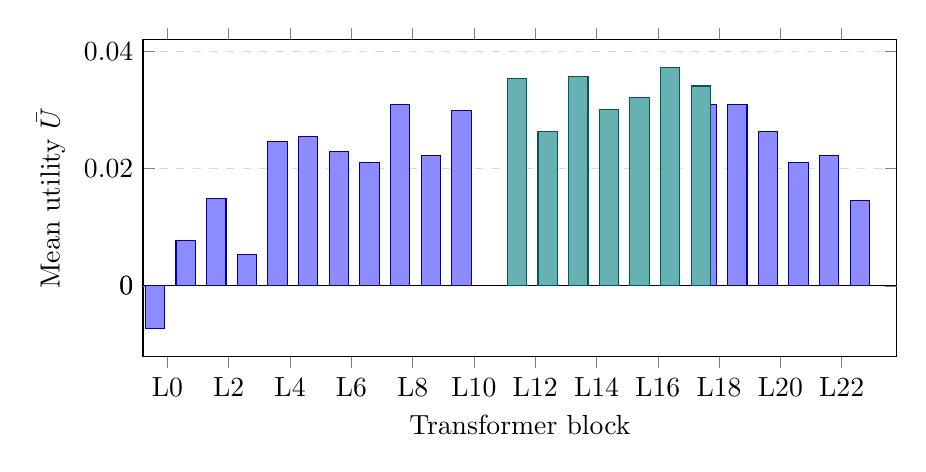
\begin{tikzpicture}
\begin{axis}[
    width=0.92\textwidth, height=5.6cm,
    ybar, bar width=7pt,
    xlabel={Transformer block}, ylabel={Mean utility $\bar U$},
    xtick={0,2,4,6,8,10,12,14,16,18,20,22},
    xticklabels={L0,L2,L4,L6,L8,L10,L12,L14,L16,L18,L20,L22},
    xmin=-0.8, xmax=23.8, ymin=-0.012, ymax=0.042,
    yticklabel style={/pgf/number format/fixed, /pgf/number format/precision=3},
    scaled y ticks=false,
    ymajorgrids=true, grid style={dashed, gray!30},
    extra y ticks={0}, extra y tick style={grid style={black, solid}},
]
\addplot[fill=blue!45, draw=blue!70!black] coordinates {
(0,-0.0073) (1,0.0077) (2,0.0149) (3,0.0053) (4,0.0246) (5,0.0255) (6,0.0230) (7,0.0210)
(8,0.0310) (9,0.0222) (10,0.0299) (18,0.0310) (19,0.0309) (20,0.0263) (21,0.0210) (22,0.0223) (23,0.0146)};
\addplot[fill=teal!60, draw=teal!70!black] coordinates {
(11,0.0354) (12,0.0263) (13,0.0357) (14,0.0301) (15,0.0322) (16,0.0372) (17,0.0341)};
\end{axis}
\end{tikzpicture}
\caption{Mean utility of each block over 3 seeds. The gain grows from L0, is highest in L11 to L17 (green) with a peak at L16 (+0.037), and drops again towards L23 (+0.015). Only L0 is below the decoder-only baseline.}
\label{fig:utility}
\end{figure*}

A few things are clear from these results. The block we adapt makes a real difference. Utility goes from $-0.007$ at L0 to $+0.037$ at L16, and every block except L0 beats the baseline. The highest mean utilities are at L16, L13, L11, L17 and L15, and the order of blocks is fairly similar across the three seeds (Kendall's $W = 0.73$).

The utility does not simply rise with depth. It rises, flattens out in the middle and then falls, like an upside-down U. A quadratic in depth explains $R^2 = 0.82$ of the variation, while a straight line explains only 0.26. L23, which is the top DSS block, comes 21st out of 24 by utility.

Single-block numbers are still uncertain. With three seeds, the median 95\% interval for one block is about $\pm 0.034$ wide, so we cannot reliably say which of two neighbouring blocks is better. The overall shape, low at the start, high in the middle and lower at the end, appears in all three seeds and also when tiles are resampled.

\section{Does DSS Predict the Gain?}

Table~\ref{tab:selectors} compares the DSS ranking and the simple rules with the measured utility order. R2 is the main DSS version used in Phase 2D and F is the Phase 2B-A ranking given above. The two give the same picture.

\begin{table}[t]
\centering
\caption{Rankings compared with measured utility. Regret is the utility lost against the best blocks, so lower is better. The Middle rule was chosen after seeing the results.}
\label{tab:selectors}
\small
\setlength{\tabcolsep}{3.5pt}
\begin{tabular}{@{}lcccc@{}}
\toprule
\textbf{Ranking} & \textbf{$\rho$} & \textbf{Partial} & \textbf{Top-1} & \textbf{Top-3} \\
\midrule
DSS (R2) & 0.420 & 0.076 & 0.015 & 0.029 \\
DSS (F) & 0.440 & 0.139 & 0.023 & 0.040 \\
MMD & $-0.077$ & 0.079 & 0.013 & 0.053 \\
Lowest-DSS & $-0.420$ & $-0.076$ & 0.045 & 0.086 \\
Early & $-0.422$ & 0 & 0.045 & 0.093 \\
Late & 0.422 & 0 & 0.023 & 0.050 \\
Middle & 0.632 & 0.728 & 0.002 & 0.017 \\
Random & 0.003 & n/a & 0.011 & 0.034 \\
\bottomrule
\end{tabular}
\end{table}

\begin{figure}[t]
\centering
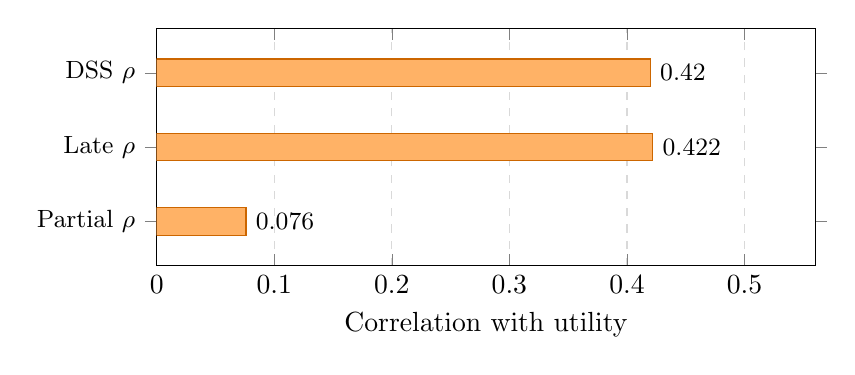
\begin{tikzpicture}
\begin{axis}[
    width=0.82\columnwidth, height=4.6cm,
    xbar, bar width=10pt,
    xlabel={Correlation with utility},
    ytick={0,1,2},
    yticklabels={{Partial $\rho$}, {Late $\rho$}, {DSS $\rho$}},
    y tick label style={font=\small},
    xmin=0, xmax=0.56,
    nodes near coords, nodes near coords style={font=\small, /pgf/number format/fixed, /pgf/number format/precision=3},
    xmajorgrids=true, grid style={dashed, gray!30},
    enlarge y limits=0.3,
]
\addplot[fill=orange!60, draw=orange!80!black] coordinates {(0.076,0) (0.422,1) (0.420,2)};
\end{axis}
\end{tikzpicture}
\caption{DSS correlates with utility about as much as the Late rule, and almost not at all once depth is removed.}
\label{fig:corr}
\end{figure}

\subsection{DSS is mostly depth}

The DSS order has a Spearman correlation of 0.420 with utility. The Late rule, which just ranks deeper blocks higher, gets 0.422. The gap between them is $-0.002$, with a tile-resampled 95\% interval of $-0.029$ to $+0.044$, so they are effectively the same (Figure~\ref{fig:corr}). After removing depth from both DSS and utility, the partial correlation is only 0.076. Whatever DSS says about utility, block depth already says it.

\subsection{Top-$k$ picks are no better than random}

Our failure test compares the DSS picks with random picks of the same size. Out of 20,000 random picks, the share that did at least as well as DSS was 0.67 for $k = 1$, 0.37 for $k = 3$ and 0.61 for $k = 5$. So DSS sits in the middle of the random results, and for $k = 1$ and $k = 5$ it is a little worse than the median random pick. The mean utility of the DSS top-$k$ blocks minus the mean of all 24 blocks is $-0.002$, $+0.003$ and $-0.001$ for $k = 1$, 3 and 5, which is no different from an average block.

\subsection{DSS picks the falling part of the curve}

Since DSS follows depth, it puts L19 to L23 at the top, and these are the blocks where utility is already going down. The top DSS block under R2 (L22) is 0.015 below the best block (L16), and L23 is 0.023 below L16. For L23 the 95\% interval of this difference does not include zero. This also explains the Phase 2C result. The DSS pair (L23, L19) did well with two blocks because deep blocks are fairly useful, not because DSS found the most useful ones.

% =======================================================
% ============ CHAPTER 6: DISCUSSION & LIMITATIONS ======
% =======================================================
\chapter{Discussion and Limitations}
\label{ch:discussion}

\section{What the Results Mean}

The main lesson from Phase 2 is that finding a difference in the features is not the same as finding where adaptation helps. DSS does measure how differently each block sees Potsdam and Vaihingen compared with the normal spread among Potsdam images. But the scaling that lets us compare blocks is dominated by the fact that deep blocks have very little natural spread. Because of this, DSS ends up as a stand-in for depth. Depth on its own is not a good guide either, since the gain does not keep increasing with depth.

The utility curve is the most useful thing we learned. Adding LoRA to almost any single block helps, and the middle of the network (L11 to L17) helps most. One possible reason is that early blocks hold low-level patterns that every later block depends on, so changing them disturbs the whole network. The last blocks feed the fixed decoder directly and may have less room to change the features. The middle blocks may sit between these two effects. We have not tested this explanation, so we offer it only as a guess.

\begin{table}[t]
\centering
\caption{Summary of the Phase 2 evidence.}
\label{tab:summary}
\small
\begin{tabular}{@{}p{3.6cm}p{3.6cm}@{}}
\toprule
\textbf{Supported} & \textbf{Not supported} \\
\midrule
Blocks differ in utility ($-0.007$ to $+0.037$) & DSS finds the useful blocks \\
Middle blocks give the largest gains (found after the fact) & DSS top-$k$ beats random \\
One adapted block helps at 23 of 24 positions & DSS adds anything beyond depth \\
The DSS computation is repeatable & MMD is a useful alternative \\
\bottomrule
\end{tabular}
\end{table}

\section{Why We Trust the Negative Result}

Table~\ref{tab:summary} lists what the evidence supports. We are fairly confident in the negative part for four reasons. The DSS ranking, the split and the analysis code were frozen and hashed before Phase 2D started, so DSS was judged on runs it had never seen. Utility is always a same-seed difference, and we checked the starting weights and data order by hash, so lucky starts do not explain the result. The same conclusion holds for both DSS versions (R2 and F), for each seed on its own, when one seed is left out, and when tiles are resampled. Finally, no test tile was opened, so the test set can still give a fair final result.

\section{Limitations}

All results come from one backbone (Prithvi-EO-2.0-300M) and one dataset pair (Potsdam to Vaihingen, IRRG), with LoRA rank 8 on Q and V, a decoder that reads only L23, and 2,000 training steps. A different model, shift or decoder may give a different picture.

We used three seeds and five validation tiles. The interval for a single block is wide (median about $\pm 0.034$), so neighbouring blocks cannot be separated and the middle-block result still needs to be confirmed on new data.

The full study covers only one adapted block at a time. Our top-$k$ comparisons combine single-block runs that were trained separately. Joint training of two blocks was done only for four rules with a single seed.

We have not yet compared against LoRA in all blocks or against full fine-tuning, so the second part of our original hypothesis, that selective adaptation can match them with fewer parameters, is still untested.

All numbers are validation results. The test tiles will be used once, for the final method only.

Lastly, the Middle rule was found after looking at the results. Its good numbers in Table~\ref{tab:selectors} do not count as evidence for any claim we registered in advance.

% =======================================================
% ============ CHAPTER 7: CONCLUSION ====================
% =======================================================
\chapter{Conclusion and Future Work}
\label{ch:conclusion}

\section{Conclusion}

In this report we described the design, checking and first full test of DSSA, a way of choosing which blocks of a geospatial foundation model to adapt with LoRA without using labels. Our findings so far are as follows.

Which block is adapted matters. Adding LoRA to one block raises the Vaihingen validation mIoU from a decoder-only mean of 0.518 up to 0.555 at L16, and the size of the gain depends a lot on the block. The gain is small for the first blocks, largest for the middle blocks (L11 to L17) and smaller again for the last ones.

In its current form, DSS is basically a depth ranking. It correlates 0.94 with depth, its correlation with utility (0.420) is the same as the Late rule (0.422), and after removing depth only 0.076 is left. The blocks it picks are no better than random picks at $k = 1$, 3 and 5. By the failure test we set at the start, the original DSSA hypothesis is not supported for the part we have tested.

The experiments themselves were carried out carefully. All 75 Phase 2D runs passed every check, every comparison is made within the same seed, and the test set has not been touched.

\section{Future Work}

The next phase follows from these results, and we will write down and freeze each step before running it.

First, we will build a version of DSS with the depth trend removed and test it, together with a fixed middle-block rule, on new seeds and data. Second, we will repeat the single-block study on a different transfer, for example Vaihingen to Potsdam or a dataset like LoveDA \cite{wang2021loveda}, to see whether the utility curve and the ranking results hold. Third, we will train jointly chosen pairs of blocks with several seeds and compare them with LoRA in all 24 blocks. Fourth, we will add full fine-tuning and measure accuracy, trainable parameters, memory and training time, so that any claim about efficiency rests on measured numbers. Only after that will we open the locked test tiles, once, for the final method.

% =======================================================
% ==================== REFERENCES =======================
% =======================================================
\small
\setstretch{1.0}
\bibliographystyle{plainnat}
\begin{thebibliography}{50}
\setlength{\itemsep}{1pt}

\bibitem[Ben-David et~al.(2010)]{bendavid2010theory}
Ben-David, S., Blitzer, J., Crammer, K., Kulesza, A., Pereira, F., and Vaughan, J.~W. (2010).
A theory of learning from different domains.
\emph{Machine Learning}, 79(1--2):151--175.

\bibitem[Cong et~al.(2022)]{cong2022satmae}
Cong, Y., Khanna, S., Meng, C., Liu, P., Rozi, E., He, Y., Burke, M., Lobell, D.~B., and Ermon, S. (2022).
SatMAE: Pre-training transformers for temporal and multi-spectral satellite imagery.
In \emph{NeurIPS}.

\bibitem[Dosovitskiy et~al.(2021)]{dosovitskiy2021image}
Dosovitskiy, A., Beyer, L., Kolesnikov, A., et~al. (2021).
An image is worth 16x16 words: Transformers for image recognition at scale.
In \emph{ICLR}.

\bibitem[Ganin et~al.(2016)]{ganin2016domain}
Ganin, Y., Ustinova, E., Ajakan, H., Germain, P., Larochelle, H., Laviolette, F., Marchand, M., and Lempitsky, V. (2016).
Domain-adversarial training of neural networks.
\emph{Journal of Machine Learning Research}, 17(59):1--35.

\bibitem[Gretton et~al.(2012)]{gretton2012kernel}
Gretton, A., Borgwardt, K.~M., Rasch, M.~J., Sch{\"o}lkopf, B., and Smola, A. (2012).
A kernel two-sample test.
\emph{Journal of Machine Learning Research}, 13:723--773.

\bibitem[He et~al.(2022)]{he2022masked}
He, K., Chen, X., Xie, S., Li, Y., Doll{\'a}r, P., and Girshick, R. (2022).
Masked autoencoders are scalable vision learners.
In \emph{Proceedings of the IEEE/CVF CVPR}, pages 16000--16009.

\bibitem[Houlsby et~al.(2019)]{houlsby2019parameter}
Houlsby, N., Giurgiu, A., Jastrzebski, S., Morrone, B., de~Laroussilhe, Q., Gesmundo, A., Attariyan, M., and Gelly, S. (2019).
Parameter-efficient transfer learning for NLP.
In \emph{ICML}, pages 2790--2799.

\bibitem[Hu et~al.(2022)]{hu2022lora}
Hu, E.~J., Shen, Y., Wallis, P., Allen-Zhu, Z., Li, Y., Wang, S., Wang, L., and Chen, W. (2022).
LoRA: Low-rank adaptation of large language models.
In \emph{ICLR}.

\bibitem[Jakubik et~al.(2023)]{jakubik2023foundation}
Jakubik, J., Roy, S., Phillips, C.~E., et~al. (2023).
Foundation models for generalist geospatial artificial intelligence.
\emph{arXiv preprint arXiv:2310.18660}.

\bibitem[Kornblith et~al.(2019)]{kornblith2019similarity}
Kornblith, S., Norouzi, M., Lee, H., and Hinton, G. (2019).
Similarity of neural network representations revisited.
In \emph{ICML}, pages 3519--3529.

\bibitem[Lee et~al.(2023)]{lee2023surgical}
Lee, Y., Chen, A.~S., Tajwar, F., Kumar, A., Yao, H., Liang, P., and Finn, C. (2023).
Surgical fine-tuning improves adaptation to distribution shifts.
In \emph{ICLR}.

\bibitem[Long et~al.(2015)]{long2015fully}
Long, J., Shelhamer, E., and Darrell, T. (2015).
Fully convolutional networks for semantic segmentation.
In \emph{Proceedings of the IEEE CVPR}, pages 3431--3440.

\bibitem[Loshchilov and Hutter(2019)]{loshchilov2019decoupled}
Loshchilov, I. and Hutter, F. (2019).
Decoupled weight decay regularization.
In \emph{ICLR}.

\bibitem[Milletari et~al.(2016)]{milletari2016vnet}
Milletari, F., Navab, N., and Ahmadi, S.-A. (2016).
V-Net: Fully convolutional neural networks for volumetric medical image segmentation.
In \emph{International Conference on 3D Vision (3DV)}, pages 565--571.

\bibitem[Raghu et~al.(2017)]{raghu2017svcca}
Raghu, M., Gilmer, J., Yosinski, J., and Sohl-Dickstein, J. (2017).
SVCCA: Singular vector canonical correlation analysis for deep learning dynamics and interpretability.
In \emph{NeurIPS}.

\bibitem[Rottensteiner et~al.(2012)]{rottensteiner2012isprs}
Rottensteiner, F., Sohn, G., Jung, J., Gerke, M., Baillard, C., Benitez, S., and Breitkopf, U. (2012).
The ISPRS benchmark on urban object classification and 3D building reconstruction.
\emph{ISPRS Annals of the Photogrammetry, Remote Sensing and Spatial Information Sciences}, I-3:293--298.

\bibitem[Szwarcman et~al.(2024)]{szwarcman2024prithvi}
Szwarcman, D., Roy, S., Fraccaro, P., et~al. (2024).
Prithvi-EO-2.0: A versatile multi-temporal foundation model for Earth observation applications.
\emph{arXiv preprint arXiv:2412.02732}.

\bibitem[Tuia et~al.(2016)]{tuia2016domain}
Tuia, D., Persello, C., and Bruzzone, L. (2016).
Domain adaptation for the classification of remote sensing data: An overview of recent advances.
\emph{IEEE Geoscience and Remote Sensing Magazine}, 4(2):41--57.

\bibitem[Wang et~al.(2021)]{wang2021loveda}
Wang, J., Zheng, Z., Ma, A., Lu, X., and Zhong, Y. (2021).
LoveDA: A remote sensing land-cover dataset for domain adaptive semantic segmentation.
In \emph{NeurIPS Datasets and Benchmarks Track}.

\bibitem[Yosinski et~al.(2014)]{yosinski2014transferable}
Yosinski, J., Clune, J., Bengio, Y., and Lipson, H. (2014).
How transferable are features in deep neural networks?
In \emph{NeurIPS}, pages 3320--3328.

\bibitem[Zhang et~al.(2023)]{zhang2023adalora}
Zhang, Q., Chen, M., Bukharin, A., He, P., Cheng, Y., Chen, W., and Zhao, T. (2023).
Adaptive budget allocation for parameter-efficient fine-tuning.
In \emph{ICLR}.

\end{thebibliography}

\end{document}
